\documentclass[12pt,a4paper]{article}

% ─── Page Layout ───────────────────────────────────────────────────────────────
\usepackage[a4paper, margin=0.8in, headheight=14pt]{geometry}

% ─── Fonts (XeLaTeX) ───────────────────────────────────────────────────────────
\usepackage{fontspec}
\usepackage{unicode-math}
\setmainfont{TeX Gyre Pagella}
\setmonofont[Scale=0.88]{TeX Gyre Cursor}
\setmathfont{Latin Modern Math}

% ─── Packages ──────────────────────────────────────────────────────────────────
\usepackage{xcolor}
\usepackage{colortbl}
\usepackage{titlesec}
\usepackage{enumitem}
\usepackage{tabularx}
\usepackage{booktabs}
\usepackage{array}
\usepackage{amsmath}
\usepackage{tikz}
\usetikzlibrary{shapes.geometric, arrows.meta, positioning, calc, fit, decorations.pathreplacing}
\usepackage{tcolorbox}
\tcbuselibrary{skins, breakable}
\usepackage{hyperref}
\usepackage{fancyhdr}
\usepackage{graphicx}
\usepackage{microtype}
\hyphenpenalty=10000
\exhyphenpenalty=10000
\sloppy
\usepackage{caption}
\usepackage{setspace}
\usepackage{multirow}
\usepackage{tocloft}

% ─── Q&A helper ────────────────────────────────────────────────────────────────
\newcommand{\Q}[1]{\textbf{#1}\par\noindent\ignorespaces}

% ─── Colour Palette ────────────────────────────────────────────────────────────
\definecolor{myred}{RGB}{196,30,58}
\definecolor{mydark}{RGB}{30,30,50}
\definecolor{mygreen}{RGB}{14,120,80}
\definecolor{myteal}{RGB}{0,130,140}
\definecolor{myamber}{RGB}{180,100,0}
\definecolor{mypurple}{RGB}{100,30,160}
\definecolor{mygray}{RGB}{246,247,249}
\definecolor{mgframe}{RGB}{180,185,200}
\definecolor{watermark}{RGB}{145,150,170}
\definecolor{hdrred}{RGB}{250,232,235}
\definecolor{hdrgreen}{RGB}{220,244,233}
\definecolor{hdrteal}{RGB}{220,242,244}
\definecolor{hdramber}{RGB}{253,242,215}
\definecolor{hdrpurple}{RGB}{238,228,255}
\definecolor{hdrgray}{RGB}{238,240,245}
\definecolor{rowalt}{RGB}{250,251,253}

% ─── Section Formatting ────────────────────────────────────────────────────────
\titleformat{\section}
  {\large\bfseries\color{myred}}{\thesection.}{0.5em}{}
  [\vspace{1pt}{\color{myred}\rule{\linewidth}{0.8pt}}]
\titleformat{\subsection}
  {\normalsize\bfseries\color{myteal}}{\thesubsection}{0.5em}{}
\titlespacing*{\section}{0pt}{18pt}{7pt}
\titlespacing*{\subsection}{0pt}{11pt}{4pt}

% ─── Paragraph ─────────────────────────────────────────────────────────────────
\setlength{\parindent}{0pt}
\setlength{\parskip}{4pt}

% ─── TOC Styling ───────────────────────────────────────────────────────────────
\renewcommand{\cfttoctitlefont}{\large\bfseries\color{myred}}
\renewcommand{\cftaftertoctitle}{\par\noindent{\color{myred}\rule{\linewidth}{0.8pt}}}
\setlength{\cftbeforetoctitleskip}{0pt}
\setlength{\cftaftertoctitleskip}{6pt}
\renewcommand{\cftsecfont}{\normalsize\bfseries\color{mydark}}
\renewcommand{\cftsecpagefont}{\normalsize\bfseries\color{mydark}}
\renewcommand{\cftsecleader}{\cftdotfill{\cftdotsep}}
\setlength{\cftbeforesecskip}{7pt}
\renewcommand{\cftsubsecfont}{\small\color{mydark}}
\renewcommand{\cftsubsecpagefont}{\small\color{mydark}}
\setlength{\cftbeforesubsecskip}{3pt}
\setlength{\cftsubsecindent}{1.4em}

% ─── Table helpers ─────────────────────────────────────────────────────────────
\renewcommand{\arraystretch}{1.45}
\setlength{\tabcolsep}{6pt}
\arrayrulecolor{mydark}
\newcolumntype{B}[1]{>{\small\bfseries\raggedright\arraybackslash}m{#1}}
\newcolumntype{Y}{>{\small\raggedright\arraybackslash}X}
\renewcommand{\tabularxcolumn}[1]{m{#1}}

% ─── Header / Footer ───────────────────────────────────────────────────────────
\pagestyle{fancy}
\fancyhf{}
\fancyhead[L]{\small\color{myred}\textbf{PE-EC603B}\;\color{mydark}--- Bio-Medical Electronics}
\fancyhead[R]{\small\color{myteal}\textbf{Module 1 Notes}}
\fancyfoot[C]{\small\color{mydark}\thepage}
\fancyfoot[R]{\small\color{watermark}\textit{\copyright\ Biraj}}
\renewcommand{\headrulewidth}{0.5pt}
\renewcommand{\footrulewidth}{0.3pt}

% ─── Hyperref ──────────────────────────────────────────────────────────────────
\hypersetup{
  colorlinks=true, linkcolor=myteal, urlcolor=myteal,
  pdfauthor={Biraj Sarkar},
  pdftitle={PE-EC603B --- Module 1 Notes}
}

% ─── tcolorbox styles ──────────────────────────────────────────────────────────
\tcbset{
  tikzbox/.style={
    colback=mygray, colframe=mgframe, boxrule=0.6pt, arc=4pt,
    left=8pt, right=8pt, top=6pt, bottom=6pt,
    colbacktitle=mgframe, coltitle=mydark,
    fonttitle=\small\bfseries
  },
  defbox/.style={
    colback=hdrgreen, colframe=mygreen, boxrule=0.8pt, arc=4pt,
    left=9pt, right=9pt, top=6pt, bottom=6pt,
    colbacktitle=mygreen, coltitle=white,
    fonttitle=\small\bfseries
  },
  formulabox/.style={
    colback=hdrteal, colframe=myteal, boxrule=0.8pt, arc=4pt,
    left=9pt, right=9pt, top=7pt, bottom=7pt,
    colbacktitle=myteal, coltitle=white,
    fonttitle=\small\bfseries
  },
  examplebox/.style={
    colback=hdramber, colframe=myamber, boxrule=0.8pt, arc=4pt,
    left=9pt, right=9pt, top=6pt, bottom=6pt,
    colbacktitle=myamber, coltitle=white,
    fonttitle=\small\bfseries
  },
  masonbox/.style={
    colback=hdrpurple, colframe=mypurple, boxrule=0.8pt, arc=4pt,
    left=9pt, right=9pt, top=6pt, bottom=6pt,
    colbacktitle=mypurple, coltitle=white,
    fonttitle=\small\bfseries
  },
  exambox/.style={
    colback=hdrpurple, colframe=mypurple, boxrule=1pt, arc=5pt,
    left=10pt, right=10pt, top=8pt, bottom=8pt,
    colbacktitle=mypurple, coltitle=white,
    fonttitle=\bfseries,
    breakable, title after break={\textbf{Frequently Asked / Viva Questions (contd.)}}}
}
% Make all boxes breakable across pages
\tcbset{breakable}

% ─── TikZ styles ───────────────────────────────────────────────────────────────
\tikzset{
  block/.style={rectangle, draw=myteal, fill=hdrteal,
    text width=2.4cm, align=center, minimum height=0.95cm,
    font=\small, rounded corners=3pt, line width=0.7pt},
  redblock/.style={rectangle, draw=myred, fill=hdrred,
    text width=2.4cm, align=center, minimum height=0.95cm,
    font=\small, rounded corners=3pt, line width=0.7pt},
  greenblock/.style={rectangle, draw=mygreen, fill=hdrgreen,
    text width=2.4cm, align=center, minimum height=0.95cm,
    font=\small, rounded corners=3pt, line width=0.7pt},
  amberblock/.style={rectangle, draw=myamber, fill=hdramber,
    text width=2.4cm, align=center, minimum height=0.95cm,
    font=\small, rounded corners=3pt, line width=0.7pt},
  purpblock/.style={rectangle, draw=mypurple, fill=hdrpurple,
    text width=2.4cm, align=center, minimum height=0.95cm,
    font=\small, rounded corners=3pt, line width=0.7pt},
  sumjunc/.style={circle, draw=myamber, fill=hdramber,
    minimum size=0.62cm, font=\small, line width=0.8pt},
  arrow/.style={-Stealth, thick, color=mydark},
  redarrow/.style={-Stealth, thick, color=myred},
  line/.style={thick, color=mydark}
}

% ═══════════════════════════════════════════════════════════════════════════════
\begin{document}
% ═══════════════════════════════════════════════════════════════════════════════

\begin{center}
  {\LARGE\bfseries\color{myred} PE-EC603B --- Bio-Medical Electronics}\\[5pt]
  {\normalsize\color{mydark} Semester VI \quad$\bullet$\quad 3L:0T:0P \quad$\bullet$\quad 3 Credits}\\[3pt]
  {\normalsize\color{myteal}\textbf{Module 1 Exam Notes: Introduction to Human Physiology}}\\[3pt]
  {\small\color{mydark} CGEC \;$|$\; B.Tech ECE (2023--27) \;$|$\; \textit{Biraj Sarkar}}
\end{center}
\vspace{2pt}
\noindent{\color{myred}\rule{\linewidth}{1.5pt}}
\vspace{2pt}

\hypersetup{linkcolor=mydark}
\tableofcontents
\hypersetup{linkcolor=myteal}
\newpage

% ===============================================================================
\section{The Human Body as an Engineering System}
% ===============================================================================

The human body can be viewed as a highly complex, self-regulating biological machine. From a bio-medical electronics perspective, it is a system with sensors (sense organs), processors (nervous system and brain), actuators (muscles), and a power supply (metabolic energy from food). Understanding this system is essential for designing instruments that measure, monitor, and assist bodily functions.

\subsection{Organ Systems Overview}

\begin{tcolorbox}[defbox, title={\textbf{Definition: Organ System}}]
An \textbf{organ system} is a group of organs that work together to perform one or more physiological functions. The human body consists of 11 major organ systems, each with specific roles in maintaining homeostasis.
\end{tcolorbox}

\textbf{Major Organ Systems Relevant to Bio-Medical Electronics:}\par\noindent
\begin{tabularx}{\linewidth}{|B{3.2cm}|Y|Y|}
\hline
\textbf{System} & \textbf{\color{myteal}Primary Organs} & \textbf{\color{mygreen}Clinical Relevance} \\
\hline
\textbf{Cardiovascular} & Heart, arteries, veins, capillaries. & ECG, blood pressure, cardiac output monitoring. \\
\hline
\textbf{Respiratory} & Lungs, diaphragm, trachea, bronchi. & Spirometry, pulse oximetry, ventilator design. \\
\hline
\textbf{Nervous} & Brain, spinal cord, peripheral nerves. & EEG, EMG, nerve conduction velocity. \\
\hline
\textbf{Muscular} & Skeletal, smooth, cardiac muscle. & EMG, prosthetic limb control, physiotherapy. \\
\hline
\textbf{Renal (Urinary)} & Kidneys, ureter, bladder. & Dialysis machine design, fluid balance monitoring. \\
\hline
\textbf{Endocrine} & Pancreas, thyroid, adrenal glands. & Blood glucose monitoring, hormone assay. \\
\hline
\end{tabularx}

\subsection{Homeostasis and Feedback Control}

\begin{tcolorbox}[defbox, title={\textbf{Definition: Homeostasis}}]
\textbf{Homeostasis} is the ability of a living organism to maintain a stable internal environment despite changes in external conditions. It is achieved through continuous negative feedback loops involving sensors, control centers, and effectors.
\end{tcolorbox}

The body maintains homeostasis by regulating parameters such as body temperature ($37\pm0.5\,^{\circ}\text{C}$), blood pH ($7.35$--$7.45$), blood glucose ($70$--$100\,\text{mg/dL}$), and arterial blood pressure ($120/80\,\text{mmHg}$). Most clinical instruments are designed to monitor deviations from these normal (baseline) values.

\begin{tcolorbox}[tikzbox, title={Biological Feedback Control Loop (Homeostasis)}]
\centering
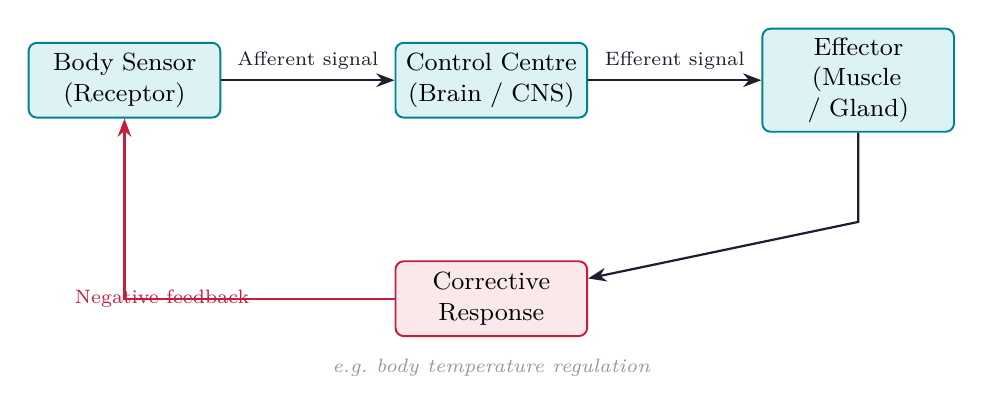
\begin{tikzpicture}[node distance=1.1cm and 2.0cm, thick]
  \node[block, text width=2.2cm] (sensor) {Body Sensor\\(Receptor)};
  \node[block, text width=2.2cm, right=2.2cm of sensor] (control) {Control Centre\\(Brain / CNS)};
  \node[block, text width=2.2cm, right=2.2cm of control] (effector) {Effector\\(Muscle / Gland)};
  \node[redblock, text width=2.2cm, below=1.8cm of control] (response) {Corrective\\Response};

  \draw[arrow] (sensor) -- node[above, font=\scriptsize, color=mydark] {Afferent signal} (control);
  \draw[arrow] (control) -- node[above, font=\scriptsize, color=mydark] {Efferent signal} (effector);
  \draw[arrow] (effector) -- ++(0,-1.8) -- (response);
  \draw[redarrow] (response) -- node[left, font=\scriptsize, color=myred] {Negative feedback} (sensor |- response) -- (sensor);

  \node[font=\scriptsize\itshape, color=watermark, below=0.15cm of response] {e.g.\ body temperature regulation};
\end{tikzpicture}
\end{tcolorbox}

% ===============================================================================
\section{The Cardiovascular System}
% ===============================================================================

The cardiovascular system (CVS) is the most extensively monitored system in bio-medical electronics, since the heart generates measurable electrical, pressure, and acoustic signals accessible from the body surface.

\subsection{Structure and Function}

\begin{tcolorbox}[defbox, title={\textbf{Definition: Cardiovascular System}}]
The \textbf{cardiovascular system} consists of the heart (pump), blood vessels (conduits), and blood (transport medium). It delivers oxygen, nutrients, and hormones to all tissues and removes metabolic waste products.
\end{tcolorbox}

The heart is a four-chambered muscular pump:
\begin{itemize}[leftmargin=*, itemsep=3pt]
  \item \textbf{Right Atrium (RA):} Receives deoxygenated blood from the body via the superior and inferior vena cava.
  \item \textbf{Right Ventricle (RV):} Pumps blood to the lungs through the pulmonary artery (pulmonary circulation).
  \item \textbf{Left Atrium (LA):} Receives oxygenated blood from the lungs via pulmonary veins.
  \item \textbf{Left Ventricle (LV):} Pumps oxygenated blood to the entire body through the aorta (systemic circulation). The LV wall is thickest because it works against the highest pressure.
\end{itemize}

\subsection{The Cardiac Cycle and Electrical Conduction}

Each heartbeat is initiated by the \textbf{Sinoatrial (SA) node} --- the heart's natural pacemaker located in the right atrium. The electrical impulse propagates through a defined conduction pathway:

\textbf{SA Node $\to$ AV Node $\to$ Bundle of His $\to$ Left and Right Bundle Branches $\to$ Purkinje Fibres $\to$ Ventricular Myocardium}

\begin{tcolorbox}[formulabox, title={\textbf{Cardiovascular Parameters and Normal Values}}]
\renewcommand{\arraystretch}{1.3}
\begin{tabularx}{\linewidth}{B{3.8cm} X}
Heart Rate (HR) & $60$--$100\,\text{beats/min}$ (normal); $< 60$ = bradycardia; $> 100$ = tachycardia. \\[4pt]
Stroke Volume (SV) & Volume ejected per beat $\approx 70\,\text{mL}$ at rest. \\[4pt]
Cardiac Output (CO) & $CO = HR \times SV \approx 5\,\text{L/min}$ at rest. \\[4pt]
Blood Pressure (BP) & Systolic $\approx 120\,\text{mmHg}$; Diastolic $\approx 80\,\text{mmHg}$. \\[4pt]
Mean Arterial Pressure & $MAP = \displaystyle\frac{SBP + 2 \times DBP}{3} \approx 93\,\text{mmHg}$.
\end{tabularx}
\end{tcolorbox}

\subsection{The ECG Signal}

The electrocardiogram (ECG) is a recording of the electrical activity of the heart from the body surface. Each cardiac cycle produces a characteristic waveform:

\begin{tcolorbox}[tikzbox, title={ECG Waveform --- Components and Significance}]
\centering
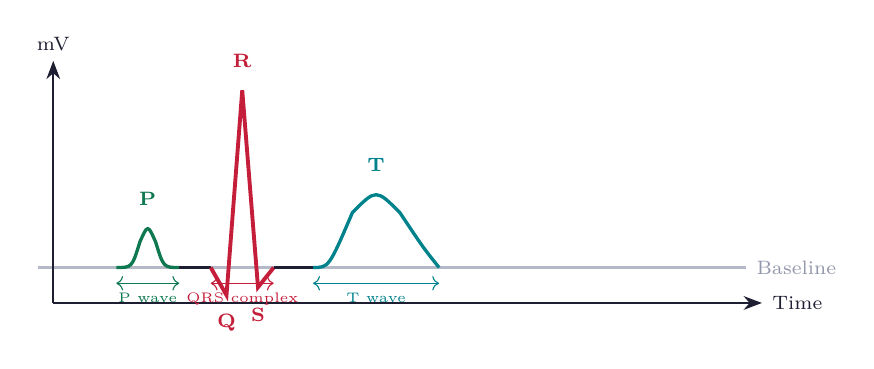
\begin{tikzpicture}[x=1.0cm, y=2.5cm, thick]
  % Baseline
  \draw[line, color=mgframe] (-0.5, 0) -- (8.5, 0) node[right, font=\scriptsize, color=watermark] {Baseline};
  % Time axis
  \draw[arrow] (-0.3, -0.18) -- (8.7, -0.18) node[right, font=\scriptsize] {Time};
  % Voltage axis
  \draw[arrow] (-0.3, -0.18) -- (-0.3, 1.05) node[above, font=\scriptsize] {mV};

  % P wave (small positive hump)
  \draw[color=mygreen, line width=1.2pt]
    (0.5, 0) .. controls (0.7, 0) .. (0.8, 0.13)
             .. controls (0.9, 0.22) .. (1.0, 0.13)
             .. controls (1.1, 0) .. (1.3, 0);

  % PQ segment
  \draw[color=mydark, line width=1.0pt] (1.3, 0) -- (1.7, 0);

  % QRS complex
  \draw[color=myred, line width=1.4pt]
    (1.7, 0) -- (1.9, -0.14) -- (2.1, 0.90) -- (2.3, -0.10) -- (2.5, 0);

  % ST segment
  \draw[color=mydark, line width=1.0pt] (2.5, 0) -- (3.0, 0);

  % T wave (positive, broader)
  \draw[color=myteal, line width=1.2pt]
    (3.0, 0) .. controls (3.2, 0) .. (3.5, 0.28)
             .. controls (3.8, 0.40) .. (4.1, 0.28)
             .. controls (4.4, 0.10) .. (4.6, 0);

  % Labels
  \node[font=\scriptsize\bfseries, color=mygreen] at (0.9, 0.35) {P};
  \node[font=\scriptsize\bfseries, color=myred] at (1.9, -0.28) {Q};
  \node[font=\scriptsize\bfseries, color=myred] at (2.1, 1.05) {R};
  \node[font=\scriptsize\bfseries, color=myred] at (2.3, -0.24) {S};
  \node[font=\scriptsize\bfseries, color=myteal] at (3.8, 0.52) {T};

  % Annotations
  \draw[<->, color=mygreen, thin] (0.5,-0.08) -- (1.3,-0.08) node[midway, below, font=\tiny] {P wave};
  \draw[<->, color=myred, thin] (1.7,-0.08) -- (2.5,-0.08) node[midway, below, font=\tiny] {QRS complex};
  \draw[<->, color=myteal, thin] (3.0,-0.08) -- (4.6,-0.08) node[midway, below, font=\tiny] {T wave};
\end{tikzpicture}
\end{tcolorbox}

\textbf{ECG Wave Significance:}\par\noindent
\begin{tabularx}{\linewidth}{|B{2.0cm}|Y|Y|}
\hline
\textbf{Wave} & \textbf{\color{myteal}Physiological Event} & \textbf{\color{myred}Normal Duration / Amplitude} \\
\hline
\textbf{P wave} & Atrial depolarization (SA node fires, atria contract). & $80$--$100\,\text{ms}$; $< 0.25\,\text{mV}$. \\
\hline
\textbf{PR Interval} & Time from atrial to ventricular depolarization (AV node delay). & $120$--$200\,\text{ms}$. \\
\hline
\textbf{QRS Complex} & Ventricular depolarization (ventricles contract). & $< 120\,\text{ms}$; $R$ up to $1.5\,\text{mV}$. \\
\hline
\textbf{ST Segment} & Ventricular plateau (all cells depolarized, isoelectric). & Flat at baseline. \\
\hline
\textbf{T wave} & Ventricular repolarization (ventricles relax). & $160\,\text{ms}$; $0.1$--$0.5\,\text{mV}$. \\
\hline
\end{tabularx}

% ===============================================================================
\section{The Respiratory System}
% ===============================================================================

\subsection{Structure and Function}

\begin{tcolorbox}[defbox, title={\textbf{Definition: Respiratory System}}]
The \textbf{respiratory system} is responsible for gas exchange between the body and the environment --- bringing oxygen ($\text{O}_2$) into the blood and expelling carbon dioxide ($\text{CO}_2$). It consists of the conducting airways (nose, pharynx, trachea, bronchi) and the respiratory zone (alveoli where gas exchange occurs).
\end{tcolorbox}

\textbf{Mechanics of Breathing:}
\begin{itemize}[leftmargin=*, itemsep=3pt]
  \item \textbf{Inspiration (active):} Diaphragm and external intercostals contract $\to$ thoracic cavity volume increases $\to$ intrapulmonary pressure drops below atmospheric pressure $\to$ air flows into lungs.
  \item \textbf{Expiration (passive at rest):} Diaphragm relaxes $\to$ thoracic cavity recoils $\to$ pressure rises above atmospheric $\to$ air flows out.
\end{itemize}

\subsection{Lung Volumes and Capacities}

\begin{tcolorbox}[formulabox, title={\textbf{Lung Volume Parameters}}]
\renewcommand{\arraystretch}{1.3}
\begin{tabularx}{\linewidth}{B{4.2cm} X}
Tidal Volume (TV)               & Volume inhaled/exhaled in one normal breath $\approx 500\,\text{mL}$. \\[4pt]
Inspiratory Reserve Volume (IRV)& Extra air that can be inhaled above TV $\approx 3000\,\text{mL}$. \\[4pt]
Expiratory Reserve Volume (ERV) & Extra air exhaled forcefully below TV $\approx 1100\,\text{mL}$. \\[4pt]
Residual Volume (RV)            & Air remaining after maximal expiration $\approx 1200\,\text{mL}$ (cannot be exhaled). \\[4pt]
Total Lung Capacity (TLC)       & $TLC = TV + IRV + ERV + RV \approx 5800\,\text{mL}$. \\[4pt]
Vital Capacity (VC)             & $VC = TV + IRV + ERV \approx 4600\,\text{mL}$ (measurable). \\[4pt]
FEV\textsubscript{1}           & Forced Expiratory Volume in 1 second; $\text{FEV}_1/\text{VC} > 70\%$ is normal.
\end{tabularx}
\end{tcolorbox}

\subsection{Respiratory Rate and Clinical Monitoring}

Normal respiratory rate (RR) is $12$--$20\,\text{breaths/min}$ in adults. Clinically monitored parameters include:
\begin{itemize}[leftmargin=*, itemsep=2pt]
  \item \textbf{Pulse Oximetry (SpO\textsubscript{2}):} Non-invasive measurement of blood oxygen saturation using red and infrared LEDs. Normal SpO$_2 \geq 95\%$.
  \item \textbf{Capnography (EtCO\textsubscript{2}):} Monitors exhaled $\text{CO}_2$ concentration, $\approx 35$--$45\,\text{mmHg}$ at end-expiration.
  \item \textbf{Spirometry:} Measures lung volumes and flow rates to diagnose obstructive (asthma, COPD) and restrictive disorders.
\end{itemize}

% ===============================================================================
\section{The Nervous System}
% ===============================================================================

\subsection{Organisation}

\begin{tcolorbox}[defbox, title={\textbf{Definition: Nervous System}}]
The \textbf{nervous system} is the body's primary communication and control network. It collects sensory information, processes it, and coordinates responses. It is divided into the \textbf{Central Nervous System (CNS)} --- brain and spinal cord --- and the \textbf{Peripheral Nervous System (PNS)} --- all nerves outside the CNS.
\end{tcolorbox}

\subsection{The Neuron and Action Potential}

The basic functional unit of the nervous system is the \textbf{neuron (nerve cell)}. It consists of:
\begin{itemize}[leftmargin=*, itemsep=3pt]
  \item \textbf{Dendrites:} Short branching processes that receive incoming signals from other neurons.
  \item \textbf{Cell Body (Soma):} Contains the nucleus and integrates incoming signals.
  \item \textbf{Axon:} Long fibre that carries signals (action potentials) away from the cell body to the next neuron or effector.
  \item \textbf{Myelin Sheath:} Insulating layer (formed by Schwann cells in PNS) that speeds up signal conduction via saltatory propagation. Conduction velocity in myelinated fibres: $40$--$70\,\text{m/s}$.
\end{itemize}

\begin{tcolorbox}[formulabox, title={\textbf{The Action Potential --- Phases and Ion Movements}}]
\renewcommand{\arraystretch}{1.3}
\begin{tabularx}{\linewidth}{B{3.2cm} X}
Resting Potential & Membrane potential $\approx -70\,\text{mV}$. Inside negative due to $\text{K}^+$ leak and $\text{Na}^+$/$\text{K}^+$ pump. \\[4pt]
Depolarization & $\text{Na}^+$ channels open rapidly $\to$ $\text{Na}^+$ rushes in $\to$ membrane potential rises to $+30\,\text{mV}$. \\[4pt]
Repolarization & $\text{Na}^+$ channels inactivate; $\text{K}^+$ channels open $\to$ $\text{K}^+$ flows out $\to$ membrane repolarizes. \\[4pt]
Hyperpolarization & $\text{K}^+$ channels close slowly $\to$ brief dip below $-70\,\text{mV}$ (refractory period). \\[4pt]
All-or-Nothing Law & An action potential either fires fully or not at all; amplitude does not vary with stimulus strength.
\end{tabularx}
\end{tcolorbox}

\begin{tcolorbox}[tikzbox, title={Action Potential Waveform}]
\centering
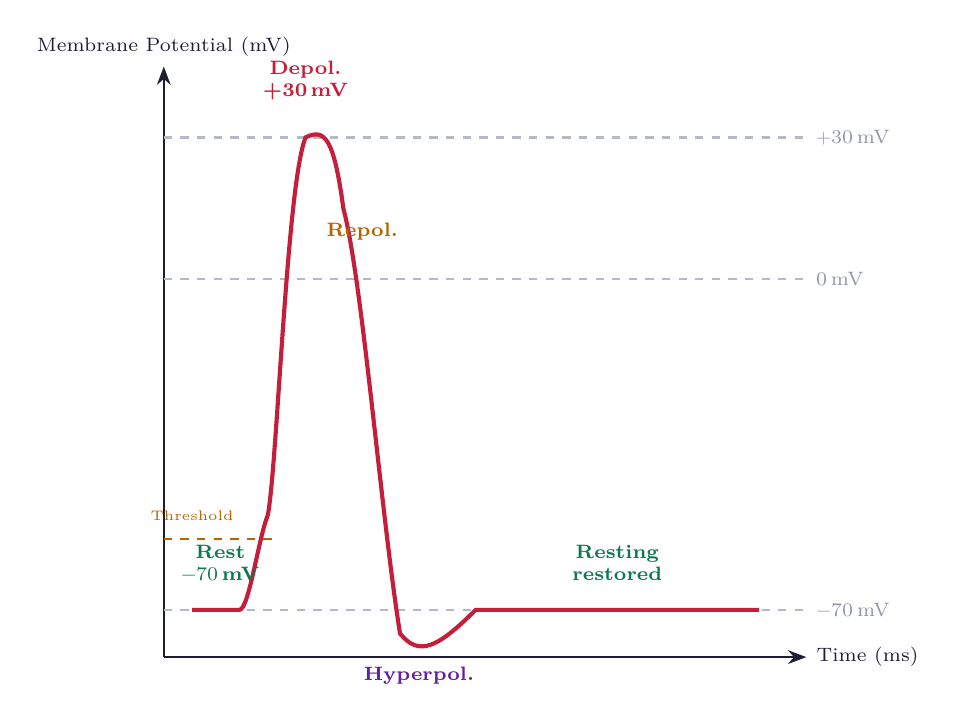
\begin{tikzpicture}[x=1.2cm, y=0.060cm, thick]
  % Axes
  \draw[arrow] (-0.3, -80) -- (6.5, -80) node[right, font=\scriptsize] {Time (ms)};
  \draw[arrow] (-0.3, -80) -- (-0.3, 45) node[above, font=\scriptsize] {Membrane Potential (mV)};

  % Resting potential line
  \draw[dashed, color=mgframe] (-0.3, -70) -- (6.5, -70) node[right, font=\scriptsize, color=watermark] {$-70\,\text{mV}$};
  \draw[dashed, color=mgframe] (-0.3, 0) -- (6.5, 0) node[right, font=\scriptsize, color=watermark] {$0\,\text{mV}$};
  \draw[dashed, color=mgframe] (-0.3, 30) -- (6.5, 30) node[right, font=\scriptsize, color=watermark] {$+30\,\text{mV}$};

  % Waveform
  \draw[color=myred, line width=1.5pt]
    (0.0, -70) -- (0.5, -70)
    .. controls (0.6, -70) and (0.7, -55) .. (0.8, -50)
    .. controls (0.9, -40) and (1.0, 20) .. (1.2, 30)
    .. controls (1.4, 32) and (1.5, 30) .. (1.6, 15)
    .. controls (1.8, 0) and (2.0, -50) .. (2.2, -75)
    .. controls (2.4, -80) and (2.6, -78) .. (3.0, -70)
    -- (6.0, -70);

  % Phase labels
  \node[font=\scriptsize\bfseries, color=mygreen, align=center] at (0.3, -60) {Rest\\\scriptsize $-70$\,mV};
  \node[font=\scriptsize\bfseries, color=myred, align=center] at (1.2, 42) {Depol.\\+30\,mV};
  \node[font=\scriptsize\bfseries, color=myamber, align=center] at (1.8, 10) {Repol.};
  \node[font=\scriptsize\bfseries, color=mypurple, align=center] at (2.4, -84) {Hyperpol.};
  \node[font=\scriptsize\bfseries, color=mygreen, align=center] at (4.5, -60) {Resting\\restored};

  % Threshold marker
  \draw[dashed, color=myamber, thin] (-0.3, -55) -- (0.85, -55);
  \node[font=\tiny, color=myamber] at (0.0, -50) {Threshold};
\end{tikzpicture}
\end{tcolorbox}

\subsection{The Brain and EEG Signals}

The brain generates rhythmic electrical activity that can be recorded as an \textbf{Electroencephalogram (EEG)} from scalp electrodes. Different frequency bands correspond to different states of consciousness:

\par\noindent
\begin{tabularx}{\linewidth}{|B{2.2cm}|>{\centering\arraybackslash}m{2.2cm}|>{\centering\arraybackslash}m{2.2cm}|Y|}
\hline
\textbf{Wave} & \textbf{\color{myteal}Freq. (Hz)} & \textbf{\color{myamber}Amplitude ($\mu$V)} & \textbf{State} \\
\hline
\textbf{Delta ($\delta$)} & 0.5 -- 4 & 20 -- 200 & Deep sleep (slow-wave sleep). \\
\hline
\textbf{Theta ($\theta$)} & 4 -- 8 & 20 -- 100 & Drowsiness, light sleep, creativity. \\
\hline
\textbf{Alpha ($\alpha$)} & 8 -- 13 & 20 -- 60 & Relaxed wakefulness, eyes closed. \\
\hline
\textbf{Beta ($\beta$)} & 13 -- 30 & 5 -- 30 & Active thinking, concentration, alert. \\
\hline
\textbf{Gamma ($\gamma$)} & 30 -- 100 & $< 10$ & Intense cognitive processing. \\
\hline
\end{tabularx}

% ===============================================================================
\section{The Muscular System and Bio-Electrical Signals Summary}
% ===============================================================================

\begin{tcolorbox}[defbox, title={\textbf{Types of Muscle Tissue}}]
\begin{itemize}[leftmargin=*, itemsep=2.5pt, topsep=0pt]
  \item \textbf{Skeletal Muscle:} Voluntary, striated, attached to bones. Controlled by the somatic nervous system. Generates \textbf{EMG} signals.
  \item \textbf{Cardiac Muscle:} Involuntary, striated, forms the heart wall. Self-excitable via SA node. Generates \textbf{ECG} signals.
  \item \textbf{Smooth Muscle:} Involuntary, non-striated, found in blood vessel walls, digestive tract, lungs. Controlled by the autonomic nervous system.
\end{itemize}
\end{tcolorbox}

\subsection{Summary of Bio-Electrical Signals}

\par\noindent
\begin{tabularx}{\linewidth}{|B{2.0cm}|Y|>{\centering\arraybackslash}m{2.2cm}|>{\centering\arraybackslash}m{2.6cm}|}
\hline
\textbf{Signal} & \textbf{\color{myteal}Physiological Origin} & \textbf{\color{myamber}Amplitude} & \textbf{\color{mygreen}Frequency Range} \\
\hline
\textbf{ECG} & Cardiac muscle depolarization/repolarization. & 0.5 -- 4 mV & 0.05 -- 150 Hz \\
\hline
\textbf{EMG} & Skeletal muscle fibre action potentials (motor units). & 0.1 -- 5 mV & 5 -- 2000 Hz \\
\hline
\textbf{EEG} & Aggregate cortical neuron activity (brain). & 5 -- 300 $\mu$V & 0.5 -- 100 Hz \\
\hline
\textbf{EOG} & Retinal dipole movement with eye motion. & 0.5 -- 1 mV & DC -- 100 Hz \\
\hline
\textbf{ERG} & Retinal response to light stimulation. & 0.5 -- 1 mV & DC -- 50 Hz \\
\hline
\textbf{EGG} & Gastro-intestinal smooth muscle electrical activity. & 0.1 -- 1 mV & 0.05 -- 1 Hz \\
\hline
\end{tabularx}

\newpage
% ===============================================================================
% MANDATORY QUICK REVISION PAGE
% ===============================================================================
\begin{center}
  {\large\bfseries\color{myred} Quick Revision --- Module 1}\\[3pt]
  {\small\color{mydark} Introduction to Human Physiology $|$ PE-EC603B}
\end{center}
\noindent{\color{myred}\rule{\linewidth}{1.2pt}}
\vspace{4pt}

\begin{tcolorbox}[formulabox, title={\textbf{Key Formulas and Normal Values}}]
\renewcommand{\arraystretch}{1.3}
\begin{tabularx}{\linewidth}{B{4.0cm} X}
Cardiac Output & $CO = HR \times SV$ \quad ($\approx 5\,\text{L/min}$ at rest) \\[4pt]
Mean Arterial Pressure & $MAP = \displaystyle\frac{SBP + 2\times DBP}{3}$ \\[8pt]
Total Lung Capacity & $TLC = TV + IRV + ERV + RV \approx 5800\,\text{mL}$ \\[4pt]
Vital Capacity & $VC = TV + IRV + ERV \approx 4600\,\text{mL}$ \\[4pt]
Nernst Equation (ion potential) & $E = \displaystyle\frac{RT}{zF}\ln\frac{[\text{ion}]_{\text{out}}}{[\text{ion}]_{\text{in}}}$ \\[8pt]
Resting Membrane Potential & $\approx -70\,\text{mV}$ (inside negative)
\end{tabularx}
\end{tcolorbox}

\begin{tcolorbox}[defbox, title={\textbf{One-Line Definitions}}]
\begin{itemize}[leftmargin=*, itemsep=2.5pt, topsep=0pt]
  \item \textbf{Homeostasis:} The body's ability to maintain a stable internal environment via negative feedback loops.
  \item \textbf{SA Node:} Sinoatrial node; the heart's natural pacemaker located in the right atrium; fires at $60$--$100\,\text{bpm}$.
  \item \textbf{Action Potential:} A brief, self-propagating reversal of membrane polarity ($-70$ to $+30\,\text{mV}$) that transmits nerve signals.
  \item \textbf{Cardiac Output:} Volume of blood pumped per minute by either ventricle; $CO = HR \times SV$.
  \item \textbf{Tidal Volume:} Volume of air inhaled or exhaled in one normal, quiet breath ($\approx 500\,\text{mL}$).
  \item \textbf{Vital Capacity:} Maximum volume of air a person can expire after a maximal inspiration.
  \item \textbf{Depolarization:} Rapid influx of $\text{Na}^+$ ions causing the cell membrane to become positive inside.
  \item \textbf{ECG:} Electrocardiogram; surface recording of the heart's electrical activity.
  \item \textbf{EEG:} Electroencephalogram; scalp recording of brain electrical activity.
  \item \textbf{EMG:} Electromyogram; recording of skeletal muscle electrical activity.
\end{itemize}
\end{tcolorbox}

\begin{tcolorbox}[exambox, title={\textbf{Frequently Asked / Viva Questions}}]
\begin{enumerate}[topsep=0pt, label=\textbf{Q\arabic*.}, itemsep=5pt]
  \item \Q{What is homeostasis? Give an example.}
    Homeostasis is the maintenance of a stable internal environment through negative feedback. Example: If body temperature rises, sweat glands are activated to cool the body back to $37\,^{\circ}\text{C}$.
  \item \Q{Describe the role of the SA node in the heart.}
    The SA node is the natural cardiac pacemaker located in the right atrium. It spontaneously depolarizes at $60$--$100\,\text{bpm}$, initiating an electrical impulse that propagates to the AV node, bundle of His, and Purkinje fibres, triggering coordinated ventricular contraction.
  \item \Q{What physiological event does the QRS complex of the ECG represent?}
    The QRS complex represents ventricular depolarization --- the electrical event that triggers the simultaneous contraction of the left and right ventricles.
  \item \Q{Define cardiac output and state its normal value.}
    Cardiac Output (CO) is the volume of blood ejected by one ventricle per minute: $CO = HR \times SV \approx 5\,\text{L/min}$ at rest for an adult.
  \item \Q{What is the difference between systolic and diastolic blood pressure?}
    Systolic pressure ($\approx 120\,\text{mmHg}$) is the peak pressure in the arteries during ventricular contraction. Diastolic pressure ($\approx 80\,\text{mmHg}$) is the minimum pressure during ventricular relaxation.
  \item \Q{Explain the all-or-nothing law of nerve conduction.}
    Once a stimulus exceeds the threshold (about $-55\,\text{mV}$), a full action potential of fixed amplitude is triggered. A sub-threshold stimulus produces no action potential at all. The amplitude does not increase with stronger stimuli.
  \item \Q{List the EEG wave bands and their corresponding brain states.}
    Delta ($0.5$--$4\,\text{Hz}$): deep sleep; Theta ($4$--$8\,\text{Hz}$): drowsiness; Alpha ($8$--$13\,\text{Hz}$): relaxed wakefulness; Beta ($13$--$30\,\text{Hz}$): active alertness; Gamma ($>30\,\text{Hz}$): intense cognition.
  \item \Q{What is the difference between ECG, EMG, and EEG signals in terms of amplitude and frequency?}
    ECG: $0.5$--$4\,\text{mV}$, $0.05$--$150\,\text{Hz}$ (cardiac). EMG: $0.1$--$5\,\text{mV}$, $5$--$2000\,\text{Hz}$ (skeletal muscle). EEG: $5$--$300\,\mu\text{V}$, $0.5$--$100\,\text{Hz}$ (brain) --- much smaller amplitude than ECG or EMG.
  \item \Q{What is the role of the myelin sheath in nerve conduction?}
    The myelin sheath acts as an electrical insulator around the axon. Depolarization jumps between nodes of Ranvier (saltatory conduction), dramatically increasing conduction velocity to $40$--$70\,\text{m/s}$ compared to $0.5$--$2\,\text{m/s}$ in unmyelinated fibres.
  \item \Q{Define tidal volume and vital capacity.}
    Tidal Volume (TV) is the volume of air inhaled/exhaled per normal breath ($\approx 500\,\text{mL}$). Vital Capacity (VC) is the maximum air that can be expelled after maximum inhalation ($VC = TV + IRV + ERV \approx 4600\,\text{mL}$).
  \item \Q{Why is the left ventricular wall thicker than the right?}
    The left ventricle pumps blood through the systemic circulation (entire body), working against a much higher resistance (pressure $\approx 120\,\text{mmHg}$). The right ventricle only pumps to the lungs (pulmonary pressure $\approx 25\,\text{mmHg}$), so it needs less force.
\end{enumerate}
\end{tcolorbox}

\begin{tcolorbox}[tikzbox, title={Bio-Electrical Signal Comparison}]
\renewcommand{\arraystretch}{1.4}
\par\noindent
\begin{tabularx}{\linewidth}{|B{1.8cm}|>{\small\centering\arraybackslash}X|>{\small\centering\arraybackslash}X|>{\small\centering\arraybackslash}X|}
\hline
\textbf{Signal} & \textbf{\color{myred}ECG} & \textbf{\color{myteal}EMG} & \textbf{\color{mypurple}EEG} \\
\hline
Source & Heart muscle & Skeletal muscle & Brain cortex \\
\hline
Amplitude & 0.5 -- 4 mV & 0.1 -- 5 mV & 5 -- 300 $\mu$V \\
\hline
Bandwidth & 0.05 -- 150 Hz & 5 -- 2000 Hz & 0.5 -- 100 Hz \\
\hline
Electrodes & Surface, chest & Surface/needle & Scalp (10-20 system) \\
\hline
Clinical use & Arrhythmia, ischemia & Neuropathy, NCV & Epilepsy, sleep disorders \\
\hline
\end{tabularx}
\end{tcolorbox}

\end{document}
